\chapter{Requirements}

\minitoc

\subsubsection{Purpose}

\clearpage

\section{Use cases}
As discussed earlier, our domain is a library system. This leaves us with objects such as books, authors, employees and customers. Possible use cases would include: 
\begin{itemize}
  \item Register a new customer
  \item Register a new employee
  \item Order a new book
  \item Add a new book to the system
  \item List books in the system
  \item Search for books
  \item Place a reservation on a book
  \item Record a borrowing of a book
  \item Record a return of a book
  \item Extend a borrowing of a book
  \item Register the state of a returned book
  \item Remove a book from the library
  \item Request that a new book is ordered
  \item Export inventory
  \item Find the location of a book
  \item Generate reports
\end{itemize}

\begin{center}
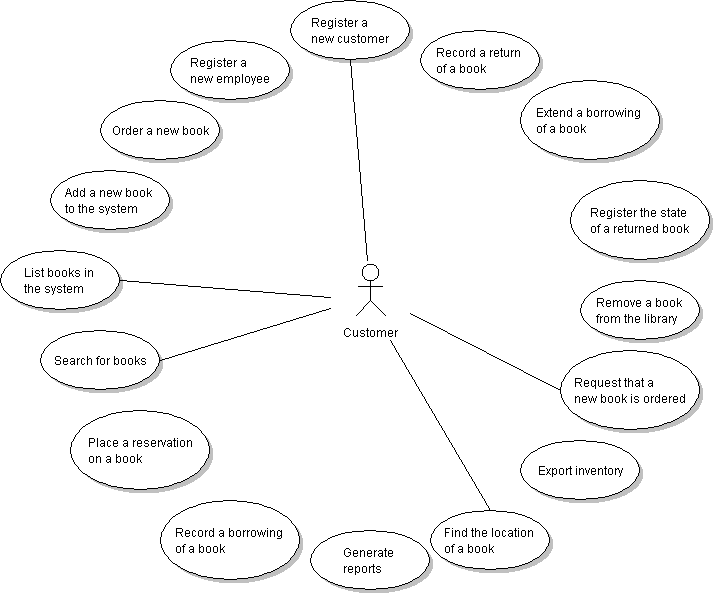
\includegraphics[width = 0.8\textwidth]{image/usecase-customer.png}
\captionof{figure}{Use Case Diagram - Customer}\label{usecase-customer}%
\end{center}

\begin{center}
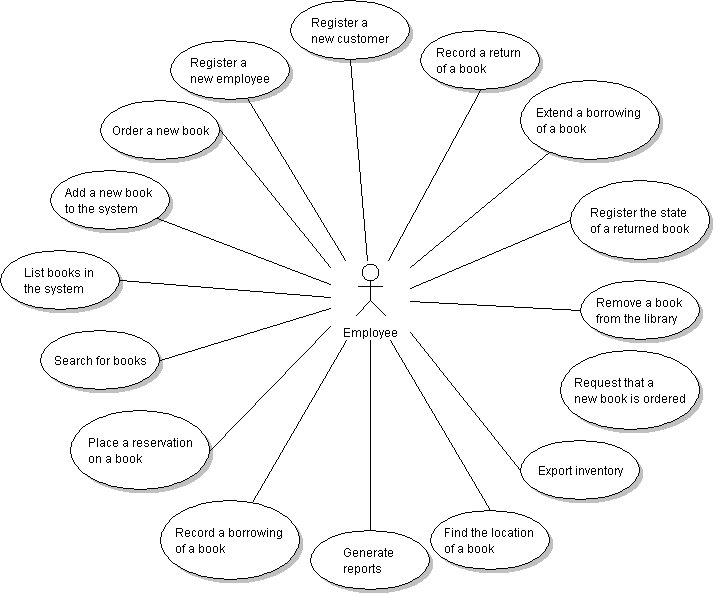
\includegraphics[width = 0.8\textwidth]{image/usecase-employee.png}
\captionof{figure}{Use Case Diagram - Employee}\label{usecase-employee}%
\end{center}

\section{User stories}
User stories are sentences describing requirements of users and justification of those requirements. They are written in the perspective of the end user. Our customer was unable to supply us with an explicit set of such user stories, so we composed a list of candidate user stories from our common understanding of the system gained through earlier meetings with the customer. The user stories are presented from a few different points of view: The administrator section describes detailed technical requirements. The general section contains stories applicable on general problems. The domain specific section contains user stories that are specific to the library domain. \footnote{http://scrummethodology.com/scrum-user-stories/}

\subsection*{Administrator point of view}
\begin{itemize}
  \item [\textbf{A1}] As an administrator, I want to be able to store objects in a persistent database, so that I can migrate data easily.
  \item [\textbf{A2}] As an administrator, I want to reflect the changes in persistent storage back to user sessions within one second, so the users always see the latest updated data.
  \item [\textbf{A3}] As an administrator, I want to be able to work directly with object attributes rather than any form of raw data.
\end{itemize}

\subsection*{User point of view - General}
\begin{itemize}
  \item [\textbf{G1}] As a user, I want my saved actions to be replicated on to the server within one second, so that my actions will not be lost and the client and server is consistent
  \item [\textbf{G2}] As a user, I want my changes to be propagated to other users of the system real- time
  \item [\textbf{G3}] As a user, I want to be able to see the console and graphical interface at the same time, so that I can use them both side by side simultaneously.
  \item [\textbf{G4}] As a user, I want the changes in console reflect in graphical user interface and likewise, so that I can have overview of the changes I made and I can understand easily, how the system works. In addition this will ensure consistency between the console and graphical interface.
  \item [\textbf{G5}] As a user, I want access to a tutorial, so that I can learn to work with the system easily.
  \item [\textbf{G6}] As a user, I want to be able to display the currently available commands in the console, so I can easily see what I can do with the objects at hand.
  \item [\textbf{G7}] As a user, I want to be able to easily repeat and edit last command, so that I can use it on another object.
  \item [\textbf{G8}] As a user, I want to be able to use batch commands, so that I can work with more than one object at the same time.
\end{itemize}

\subsection*{User point of view - Domain specific}
\begin{itemize}
  \item [\textbf{D1}] As a user, I want to be able to add a new book to the system using both the console and graphical interface.
  \item [\textbf{D2}] As a user, I want to be able to delete a book in the system using both the console and graphical interface.
  \item [\textbf{D3}] As a user, I want to be able to edit information on a specific book and save these changes using both the console and graphical interface.
  \item [\textbf{D4}] As a user, I want to be able to search for a specific book in the system, so that I can watch the information on it using both the console and graphical interface.
  \item [\textbf{D5}] As a user, I want to be able to list all the books currently in the system, so that I easily can get an overview of all the books currently in the library. This should be possible in both the console and the graphical interface.
  \item [\textbf{D6}] As a user, I want to be able to register a new customer in the system, so that customers can be saved in the system. This should be possible in both the console and the graphical interface.
  \item [\textbf{D7}] As a user, I want to be able to registrate when a customer borrows a book, so that the information is stored in the system. This should be possible in both the console and the graphical interface.
  \item [\textbf{D8}] As a user, I want to be able to edit the information on a specific borrowing of a book, so that any changes can be recorded. This should be possible in both the console and the graphical interface.
  \item [\textbf{D9}] As a user, I want to be able to list all the books currently borrowed, so that I can get information on each of them. This should be possible in both the console and the graphical interface.
  \item [\textbf{D10}] As a user, I want to be able to reserve a book for a customer, so that customers can request and reserve certain books. This should be possible in both the console and the graphical interface.
  \item [\textbf{D11}] As a user, I want to be able to list all the reservations currently in the system. This should be possible in both the console and the graphical interface.
  \item [\textbf{D12}] As a user, I want to be able to view reservations on specific books, so that I can see if a specific book is available for borrowing at the moment. This should be possible in both the console and the graphical interface.
  \item [\textbf{D13}] As a user, I want to be able to order new books for the library using both the console and the graphical interface.
\end{itemize}


\subsection*{Difficulty Level Assignment}
We proceeded to collectively estimate the difficulty of implementing each user story, presented in Table~\ref{table:userstory-difficulty}.

\begin{table}
\begin{tabular}{ | l | l | l | }
  \hline
  \textbf{User Story} & \textbf{Difficulty Level} & \textbf{Description} \\ \hline
  A1 & 5 			& Database persistence \\ \hline
  A2 & 6 			& Real time server synchronization \\ \hline
  A3 & 4 			& Exposing objects rather than raw data \\ \hline
  D1 & 1 (reference) 	& Adding books \\ \hline
  D2 & 0.5 			& Deleting books \\ \hline
  D3 & 2 			& Editing books \\ \hline
  D4 & 0.75 			& Searching for books \\ \hline
  D5 & 1.5 			& Listing all books \\ \hline
  D6 & 1 			& Register new customer \\ \hline
  D7 & 1.75 			& Record when books are borrowed \\ \hline
  D8 & 2.5 			& Edit records on a borrowing of a book \\ \hline
  D9 & 2 			& List all currently borrowed books \\ \hline
  D10 & 3 			& Record book reservations \\ \hline
  D11 & 2 			& List all reservations \\ \hline
  D12 & 1.5 			& View reservations on a book \\ \hline
  D13 & 1.5 			& Order new books \\ \hline
  G1 & 3.5 			& Save users' changes to server \\ \hline
  G2 & 2 			& Save users' changes in real time \\ \hline
  G3 & 8 			& See console and web UI simultaneously \\ \hline
  G4 & 4 			& Synchronize console and web UI \\ \hline
  G5 & 3 			& Tutorial \\ \hline
  G6 & 3 			& Display available commands \\ \hline
  G7 & 2 			& Repeat previous commands \\ \hline
  G8 & 3 			& Batch commands \\ \hline
\end{tabular}
\caption{User story diffuculty}
\label{table:userstory-difficulty}
\end{table}

\subsection{Initial Backlog}
The list of user stories was reviewed by the customer and approved as an initial product backlog. We would use this list for prioritizing which functionality to implement during the planning meeting for the first sprint.